\documentclass[11pt]{aghdpl}
% \documentclass[en,11pt]{aghdpl}  % praca w języku angielskim
\usepackage[polish]{babel}
%\usepackage[english]{babel}
\usepackage[utf8]{inputenc}

% dodatkowe pakiety
\usepackage{enumerate}
\usepackage{listings}
\lstloadlanguages{TeX}

\lstset{
  literate={ą}{{\k{a}}}1
           {ć}{{\'c}}1
           {ę}{{\k{e}}}1
           {ó}{{\'o}}1
           {ń}{{\'n}}1
           {ł}{{\l{}}}1
           {ś}{{\'s}}1
           {ź}{{\'z}}1
           {ż}{{\.z}}1
           {Ą}{{\k{A}}}1
           {Ć}{{\'C}}1
           {Ę}{{\k{E}}}1
           {Ó}{{\'O}}1
           {Ń}{{\'N}}1
           {Ł}{{\L{}}}1
           {Ś}{{\'S}}1
           {Ź}{{\'Z}}1
           {Ż}{{\.Z}}1
}

%---------------------------------------------------------------------------

\author{Rafał Włodarz}
\shortauthor{R. Włodarz}

\titlePL{Algorytm sterowania wykorzystujący sztuczne sieci neuronowe dla bezzałogowego statku latającego typu TRICOPTER}
\titleEN{}

\shorttitlePL{Algorytm sterowania wykorzystujący sztuczne sieci neuronowe} % skrócona wersja tytułu jeśli jest bardzo długi
%\shorttitleEN{Thesis in \LaTeX}

\thesistype{Praca dyplomowa magisterska}
%\thesistype{Master of Science Thesis}

\supervisor{dr hab. Adam Piłat}
%\supervisor{Marcin Szpyrka PhD, DSc}

\degreeprogramme{Automatyka i robotyka}
%\degreeprogramme{Computer Science}

\date{2015}

\department{Katedra Automatyki}
%\department{Department of Applied Computer Science}

\faculty{Wydział Elektrotechniki, Automatyki,\protect\\[-1mm] Informatyki i Inżynierii Biomedycznej}
%\faculty{Faculty of Electrical Engineering, Automatics, Computer Science and Biomedical Engineering}

\acknowledgements{Serdecznie dziękuję \dots tu ciąg dalszych podziękowań np. dla promotora, żony, sąsiada itp.}


\setlength{\cftsecnumwidth}{10mm}

%---------------------------------------------------------------------------
\setcounter{secnumdepth}{4}

\begin{document}

\titlepages
\setcounter{tocdepth}{3}
\tableofcontents
\clearpage

\chapter{Wstęp}
\label{cha:wprowadzenie}

\section{Cele pracy}
\label{sec:celePracy}

\section{Zawartość pracy}
\label{sec: zawartosc_pracy}



















\chapter{Sztuczne sieci neuronowe}
\label{cha:sztuczne_sieci_neuronowe}

Rozdział ten zawiera informacje na temat sieci neuronowych, ich architektury, zasady działania oraz algorytmów uczenia.

\section{Początki sieci neuronowych}
\label{sec:poczatki_sieci_neuronowych}
Początki prac nad poznaniem procesów zachodzących w mózgu datuje się na rok 1943. W pracy McCulloch'a oraz Pitts'a przedstawiono matematyczny model neuronu, który zapoczątkował badania związane z tym tematem. W 1949 roku Donald Hebb odkrył, iż informacje przechowywane w sieci neuronowej są reprezentowane jako wartości wag pomiędzy poszczególnymi neuronami. Na podstawie tych informacji zaproponował on pierwszy algorytm uczenia sieci neuronowej, który został nazwany regułą Hebba. Już wtedy odkryto, iż bardzo dużą zaletą sieci jest równoległy sposób przetwarzania informacji oraz metodologia uczenia, która zastępuje tradycyjny proces programowania. 



\chapter{Architektura statku latającego typu tricopter}
\label{cha:architektura_statku_latajacego_typu_tricopter}

Poniższy rozdział przedstawia zbiór podstawowych zagadnień związanych z konstrukcją wirnikowca typu tricoper oraz zawiera informacje na temat zasad sterowania układem.

\section{Konstrukcja i sterowanie tricopterem}

Ze względu na skomplikowany sposób sterowanie tricopterem w przestrzeni, oraz złożoną konstrukcję w poniższym podrozdziale zostaną przedstawione podstawowe zagadnienia związane z tymi zagadnieniami.

Na rysunku \ref{fig:orientation} przedstawiono przyjętą konwencję nazewnictwa dla poszczególnych elementów tricoptera odpowiedzialnych za przemieszczanie się układu w przestrzeni. Pokazano również położenie modelu w układzie współrzędnych, które jest niezbędne do przejrzystego opisu zasad sterowania.

\begin{figure}[!htbp]
\centering
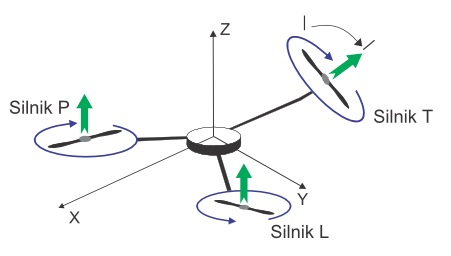
\includegraphics[width=0.7\linewidth]{./include/orientation}
\caption{Przyjęta orientacja tricoptera w układzie współrzędnych.}
\label{fig:orientation}
\end{figure}

Tricopter należy grupy rzadko spotykanych wielokomórkowców wyposażonych w nieparzystą liczbę silników odpowiadających za napędy w układzie.
Konstrukcja ta zdecydowanie utrudnia sterowanie ze względu na brak stabilności tego układu. Spowodowane jest to brakiem kompensacji siły bocznej pochodzącej od napędu niesparowanego. Czego skutkiem jest  efekt autorotacji obiektu wokół osi Z przy założeniu, iż wszystkie wirniki są w pozycji pionowej, tak jak w przypadku większości obiektów latających pionowego startu. Aby wyeliminować powyższy efekt zastosowano odpowiedni moduł składający się z serwomechanizmu, który reguluje kąt nachylenia wirnika T.


Przemieszczanie obiektu latającego w przestrzeni wymaga opracowania metodyki sterowania poszczególnymi wirnikami podczas przemieszczania się względem każdej z osi.
Bazując na poprzednim algorytmie sterującym zaprezentowano poniżej sposoby przemieszczania względem konkretnych osi tricoptera. Szczegółowe informacje związane z powyższymi zagadnieniami zostały opisane w pracy inżynierskiej autora w rozdziale 5. %TODO zrobic odnosnik do inz

\subsection{Przemieszczanie względem osi X}
Aby dokonać obrotu względem osi X konieczna jest ingerencja w ciąg wirników L oraz P. Aby uzyskać efekt przechylenia w lewą stronę konieczna jest redukcja siły ciągu na silniku L. Opcjonalnie w celu przyśpieszenia manewru można proporcjonalnie zwiększyć ciąg silnika P. Na rysunku \ref{fig:axis_x} przedstawiono opisany manewr.

\begin{figure}[!htbp]
\centering
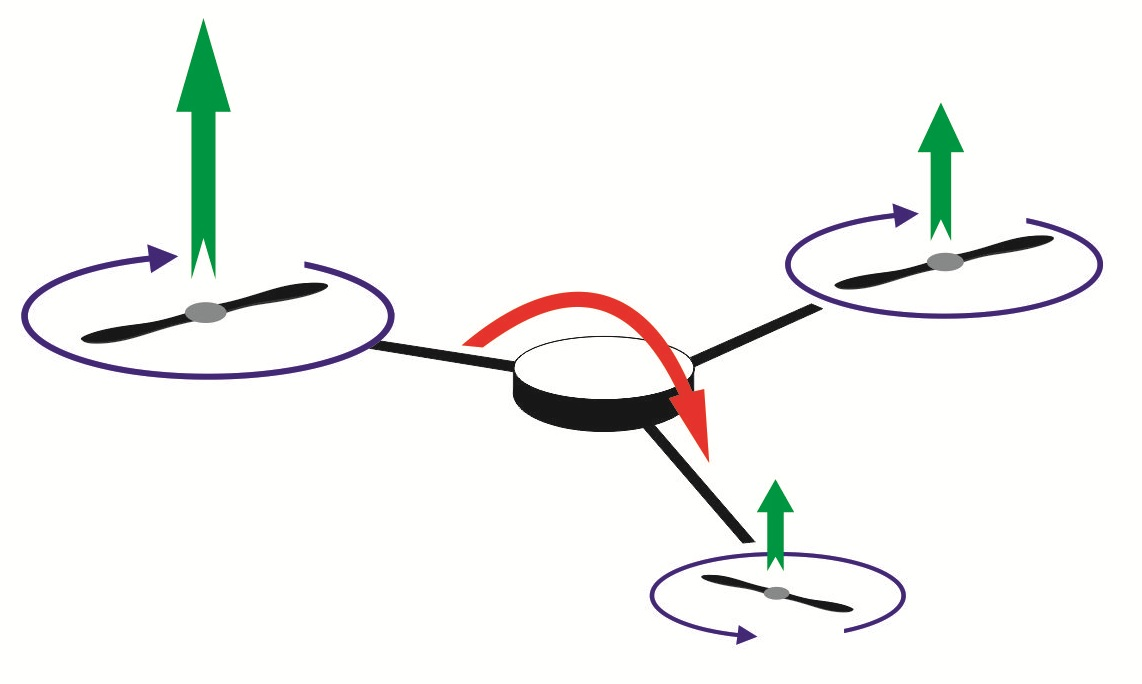
\includegraphics[width=0.7\linewidth]{./include/axis_x}
\caption{Sterowanie oraz stabilizacja w osi X.}
\label{fig:axis_x}
\end{figure}


\subsection{Przemieszczanie względem osi Y}
Obrót względem osi Y można zdecydowanie określić jako najważniejszy dla każdego obiektu latającego, odpowiada on za przemieszczenie się w przód. Odchylenie tricoptera zapewnia się przez regulację ciągu na wirniku T. Tak jak w przypadku osi X można zwiększyć prędkość obrotu obiektu przez symetrycznym modyfikacją mocy silników L oraz P wartość przeciwną co do znaku względem modyfikacji wirnika Z. Manewr ten został przedstawiony na rysunku \ref{fig:axis_y}.
\begin{figure}[!htbp]
\centering
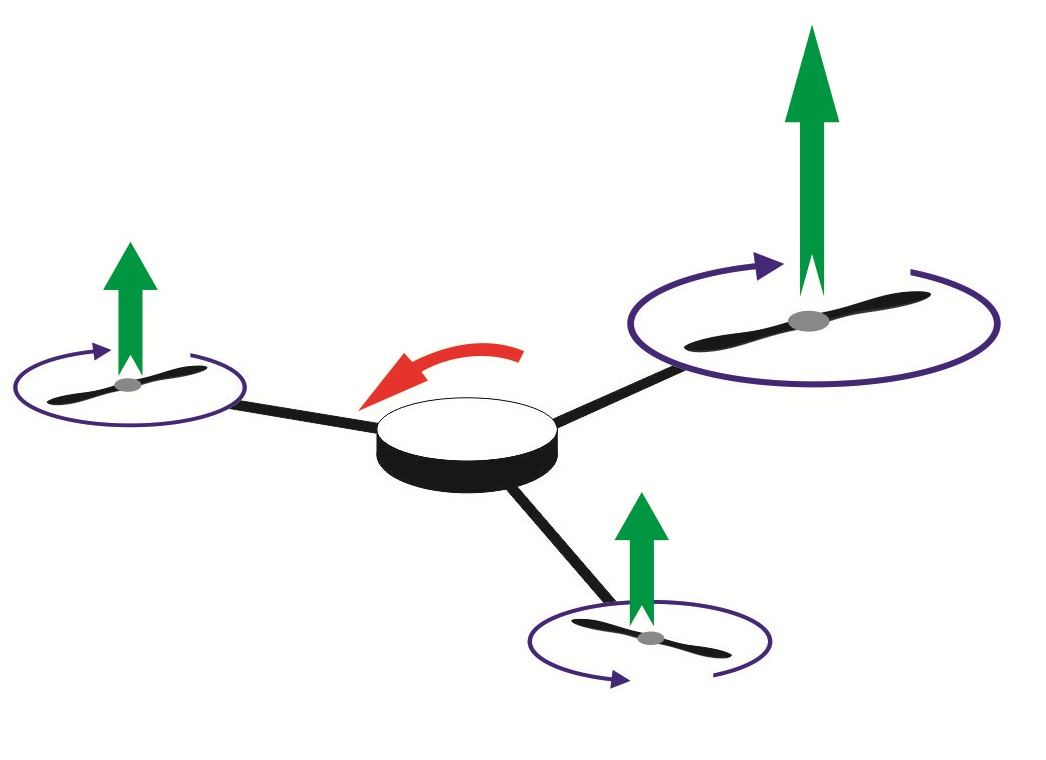
\includegraphics[width=0.7\linewidth]{./include/axis_y}
\caption{Sterowanie oraz stabilizacja w osi Y.}
\label{fig:axis_y}
\end{figure}


\subsection{Przemieszczanie względem osi Z}
Przemieszczanie względem osi Z jest głównie używane do zmiany kierunku lotu tricoptera. Manewr ten można wykonywać bez ingerencji w moc każdego z wirników. Zmiana kąta nachylenia silnika T powoduje pojawienie się efektu rotacji obiektu. Warto zwrócić uwagę, iż zbyt duże odchylenie wirnika od punktu stabilnego spowoduje również ruch tricoptera względem osi Y, ponieważ zmiana kąta nachylenia silnika Z powoduje zmianę pionowej siły ciągu, która odpowiada również za stabilizację tego obiektu. 

\begin{figure}[!htbp]
\centering
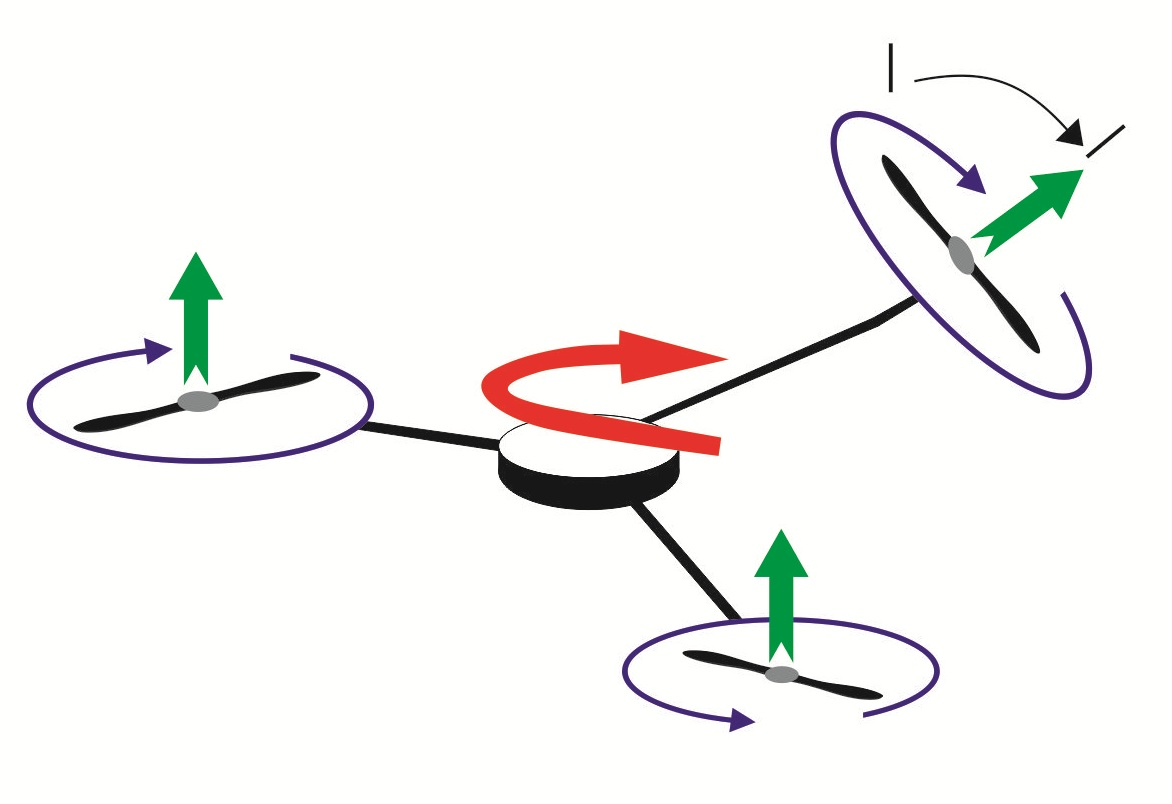
\includegraphics[width=0.7\linewidth]{./include/axis_z}
\caption{Sterowanie oraz stabilizacja w osi Z.}
\label{fig:axis_z}
\end{figure}


\section{Budowa modelu}
Ze względu na to, iż temat tej pracy bazuje na wykorzystaniu do testów gotowego obiektu latającego typu tricopter, autor zdecydował pominąć szczegółowy opis budowy modelu.
Szczegółowe informacje dotyczące konstrukcji oraz parametrów wielowirnikowca zostały przedstawione w pracy inżynierskiej autora w rozdziale 2. %TODO odnośnik do inż.




\chapter{Aplikacja sterująca}
\label{cha:aplikacja_sterujaca}
W niniejszym rozdziale przedstawiono informacje na temat aplikacji sterującej. Zagadnienia teoretyczne konieczne do zrozumienia problemu, poszczególne etapy przygotowania platformy sprzętowej, oraz proces tworzenia systemu czasu rzeczywistego.




\section{System czasu rzeczywistego}
System czasu rzeczywistego (ang. real-time system) to system, który przetwarza każdy rodzaj informacji i który musi reagować na sygnały wejściowe - bodźce generowane z zewnątrz w skończonym i określonym czasie. Jego poprawne działanie zależy zarówno od prawidłowych rezultatów logicznych, jak również od czasu reakcji.
Na podstawie tych kryteriów są one dzielone na:
\begin{itemize}
	\item Systemy o ostrych wymaganiach czasowych (ang. hard real-time) - wymagania czasowe muszą być skrupulatnie przestrzegane, naruszenie ram czasowych może wpłynąć na życie ludzkie, środowisko czy też sam system,
 
	\item Systemy o słabych wymaganiach czasowych (ang. soft real-time) – głównym kryterium oceny tych jest średni czas odpowiedzi. Sporadyczne opóźnienie nie powoduje zagrożenia lecz jedynie wpływa negatywnie na ocenę całego systemu,

	\item Systemy o solidnych wymaganiach czasowych (ang. firm real-time) - są one kombinacją systemów o wymaganiach ostrych oraz słabych. Naruszenie kryterium czasowych może pojawiać się okazjonalnie. Często dla lepszej oceny systemu stosuje się ograniczenia czasowe o charakterze "słabym" - krótsze, których przekroczenie nie powoduje katastrofy oraz "ostrym" - dłuższe, których naruszenie oznacza nieprawidłowe działanie systemu. 

\end{itemize}

Bez względu na to do której grupy systemów zalicza się aplikację musi ona charakteryzować się następującymi cechami:

\begin{itemize}
	\item Ciągłość działania - powinny działać nieprzerwanie w okresie od uruchomienia systemu do jego wycofania,
	
	\item Zależność od otoczenia - zachowanie opiera rozpatruje się w kontekście otoczenia. Prowadzone obliczenia zależą od zdarzeń oraz danych pochodzących z zewnątrz układu,
	
	\item Współbieżność - struktura systemu narzuca, aby jednoczesne zdarzenia były obsługiwane równocześnie przez szereg procesów,
	
	\item Przewidywalność - zdarzenia i dane generowane przez otoczenie pojawiają się przypadkowo co nie narusza deterministycznego zachowania systemu,
	
	\item Punktualność - odpowiedź systemu na bodźce zewnętrzne powinna być dostarczona w odpowiednich momentach - wymaganych ramach czasowych.
\end{itemize}

Z pewnością aplikacja sterująca obiektami latającymi powinna spełniać wszystkie powyższe założenia. Gdyby któreś z nich nie zostało spełnione jakiekolwiek próby sterowania zakończyły by się porażką.

Dynamika wielokomórkowców wymaga od aplikacji bardzo szybkiego czasu reakcji na zewnętrzne impulsy. Opóźnienie sterowania w takim przypadku powoduje bardzo negatywne skutki do których zaliczamy: brak kontroli nad obiektem, utrata stabilności w powietrzu oraz niekontrolowane zetknięciu się z przeszkodą. Wszystkie wymienione zachowania mogą powodować bardzo duże zniszczenia dla modelu, jego otoczenia oraz zagrażać zdrowiu operatora oraz innych osób znajdujących się w zasięgu działania modelu.

Na podstawie definicji oraz powyższej analizy skutków określono, iż aplikacja sterującą zalicza się do systemu hard-real time. 




\section{Konfiguracja beaglebone black}
Ze względu na kontynuację prac nad modelem bazowa konfiguracja beaglebone black wraz z dodatkowymi czujnikami oraz urządzeniami peryferyjnymi opisano w pracy
% TODO: inz Rwlodarz JZrebiec.

W trakcje powstawania niniejszej pracy na rynku dostępne są nowsze czujniki, które mogłyby podnieść jakość oraz częstość pomiarów, jednak ingerencja w konfigurację uniemożliwiła by porównanie algorytmów tradycyjnych z sieciami neuronowym stąd wszystkie testy zostały przeprowadzone na tej samej konfiguracji.




\section{Przygotowanie systemu operacyjnego}
Ze względu na wcześniej wspominaną specyfikę systemu sterującego oraz zastosowanie platformy sprzętowej typu mini PC wraz z systemem operacyjnym typu UNIX, ważne jest, aby wyeliminować wszelkie możliwe przerwania oraz inne aspekty, które wpływają na płynność oraz czas wykonywania się aplikacji sterującej.

Wprowadzono usprawnienie w postaci instalacji systemu operacyjnego wyposażonego w jądro czasu rzeczywistego (ang. real-time kernel). Jądro to określane jest również jako w pełni wywłaszczalne. Oznacza to, iż dopuszczane jest wywłaszczenie procesu działającego w trybie jądra. Cecha ta wraz z wcześniej narzuconymi priorytetami dla poszczególnych procesów gwarantuje, iż aplikacja sterująca, uruchomiona z wysokim priorytetem nie zostanie wywłaszczona na zbyt długi czas przez inne procesy systemowe.

Zabieg ten pozwala nam spełnić podstawową cechę systemów czasu rzeczywistego, którą jest punktualność.




\section{Tworzenie aplikacji niezależnej od platformy sprzętowej}
Dobrze zaprojektowana aplikacja sterująca obiektami latającymi powinna mieć możliwa uruchomienia na różnorodnych platformach sprzętowych, bez względu na architekturę wykorzystanych do ich budowy procesorów.

Podstawowa wersja aplikacji została poddana testom, które porównały wyniki działania sieci neuronowej na 2 całkowicie odmiennych platformach. 


\subsection{Najważniejsze aspekty}
Pierwszym, a zarazem najważniejszym aspektem jest problem, który może powstać podczas mnożenia liczb zmiennoprzecinkowych. W przypadku wykonywania tej operacji dwie liczby reprezentowane w postaci binarnej o z góry określonej liczbie dostępnych bietów o określonej liczbie bitów  wynik zapisywany jest do zmiennej o określonej liczbie bitów, co wiąże się z uzyskaniem błędu odcięcia w przypadku nie wystarczającej liczbie bitów potrzebnych do reprezentacji części ułamkowej. 



Konfiguracja miała na celu uwydatnienie problemu błędu obcięcia liczb zmiennoprzecinkowych 

\subsection{Testy}
Do testów wykorzystano komputer stacjonarny z 64 bitowym procesorem Intel i5-4670 3.40 Ghz oraz układ beaglebone black, który został wyposażony w procesor 32 bitowy ARM Cortex-A8 o częstotliwości taktowania 1GHz.

W celu uwydatnienia problemu stworzono sieć neuronową posiadającą po jednej z warstw wejściowej, ukrytej, wyjściowej. Wagi poszczególnych neuronów zostały dobrane w sposób losowy tak, jednak wszystkich z nich wykorzystują maksymalną dostępną dokładność. Następnie na wejście sieci podawana jest stała wartość. Po jej przetworzeniu otrzymujemy wynik  




\section{Architektura systemu sterującego}

\chapter{Testy systemu sterującego}
\label{cha:testy}

W tym rozdziale zostały omówione badania sieci neuronowej. Ich głównym celem jest sprawdzenie poprawności jej działania, określenie optymalnej topologii sieci oraz układu połączeń między neuronami.

\section{Testy poprawności działania sztucznej sieci neuronowej}

Ze względu na nietrywialną implementację zagadnień związanych z sieciami neuronowymi oraz algorytmów uczących, sieć została przetestowana pod kątem poprawności działania na zdecydowanie prostszym zagadnieniu jakim jest operacja logiczna typu XOR.

Została ona wybrana ze względu na łatwość zrozumienia problemu, bezproblemowe określenie oczekiwanego wyniku oraz brak wymaganego zbioru uczącego - wektor wejściowy może on zostać wygenerowany podczas samego procesu uczenia, natomiast wartość oczekiwana zostaje obliczona przy pomocy prostej operacji logicznej.

\begin{table}
\centering
\label{tab:expected_xor_output}
\begin{tabular}{|r|l|l|}
  \hline 
  Wejście 1 & Wejście 2 & Wyjście \\
  \hline 
  0 & 0 & 0 \\
  \hline
  0 & 1 & 1 \\
  \hline
  1 & 0 & 1 \\
  \hline
  1 & 1 & 0 \\
  \hline
\end{tabular}
\caption{Oczekiwane wartości odpowiedzi sieci realizującej xor.}
\end{table}

Na podstawie \ref{tab:expected_xor_output} łatwo zauważyć, iż operacja te jest nieliniowa. Cecha ta powoduje, iż pojedyńczy do realizacji tego problemu wymagana jest sieć wielowarstwowa - z przynajmniej jedną warstwą ukrytą. Do rozwiązania tego zagadnienia zastosowano dipolarną funkcję sigmoidalną - tangens hiperboliczny.
Działanie sieci neuronowej zostało sprawdzone w dwuch przypadkach. Pierwszy z nich dla niewystarczającej ilości neuronów potrzebnych do realizacji tego zagadnienia. Następnie drugi przypadek wykorzystuje odpowiednią architekturę sieci potrzebną do realizacji zagadnienia, aby wykazać poprawność działania implementacji.

\begin{figure}[!htbp]
\centering
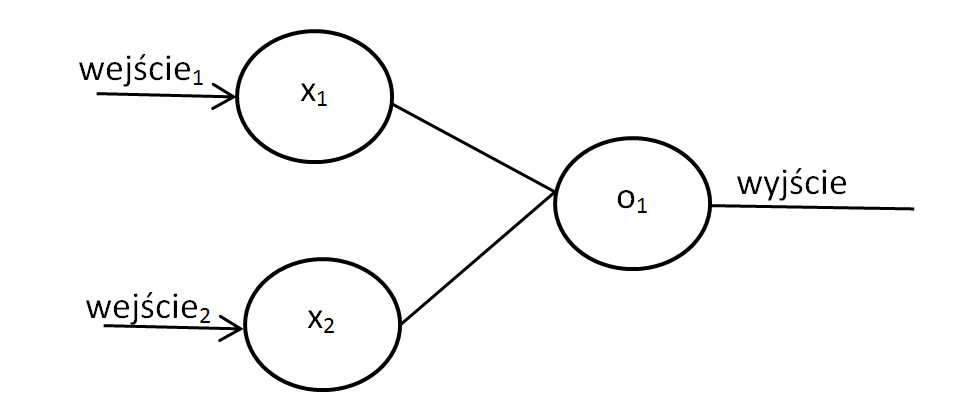
\includegraphics[width=0.7\linewidth]{./include/flow_2_1}
\caption{Przepływ informacji w topologii 2-1.}
\label{fig:flow_2_1}
\end{figure}

Na wykresie \ref{fig:neuro_2_1} przedstawiono proces uczenia sieci. Zawiera on informacje o błędach odpowiedzi sieci w poszczególnych iteracjach algorytmu uczenia.

\begin{figure}[!h]
\centering
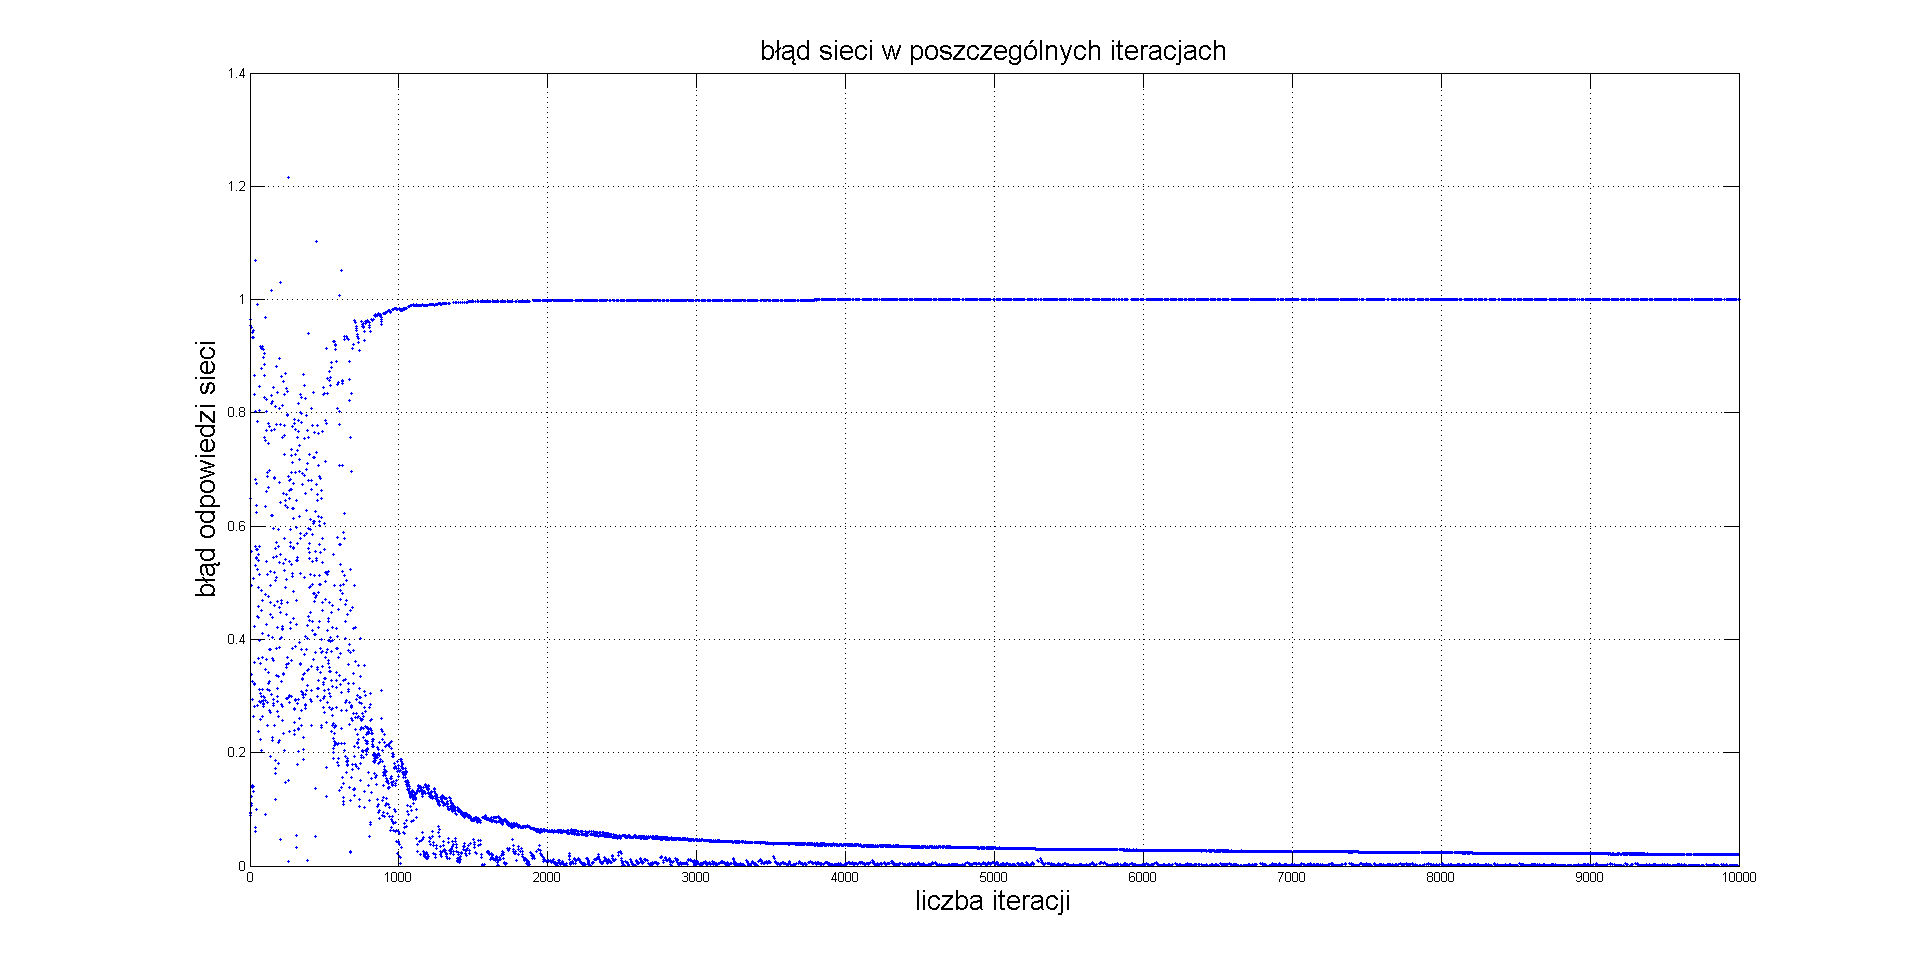
\includegraphics[width=1\linewidth]{./include/topologia_2_1}
\caption{Wykres błędu w kolejnych iteracjach dla sieci o topologii 2-1.}
\label{fig:neuro_2_1}
\end{figure}

\begin{table}
\centering

\label{tab:xor_output_2_1}
\begin{tabular}{|r|l|l|}
  \hline 
  Wejście 1 & Wejście 2 & Wyjście \\
  \hline 
  0 & 0 & 0 \\
  \hline
  0 & 1 & 1 \\
  \hline
  1 & 0 & 1 \\
  \hline
  1 & 1 & 0 \\
  \hline
\end{tabular}
\caption{Odpowiedzi sieci neuronowej o topologii 2-1.}
\end{table}

Na podstawie powyższego zestawienia: wykresu \ref{fig:neuro_2_1}, oraz tabeli \ref{tab:xor_output_2_1} można uznać, iż weryfikacja potwierdziła wcześniejszą tezę teoretyczną, która zakłada, iż sieć neuronowa nie posiadająca ukrytej warstwy nie jest w stanie rozwiązać zagadnień nieliczniowych. Jednocześnie potwierdza to, zgodność implementacji z teorią dotyczącą sieci neuronowych.

\begin{figure}[!htbp]
\centering
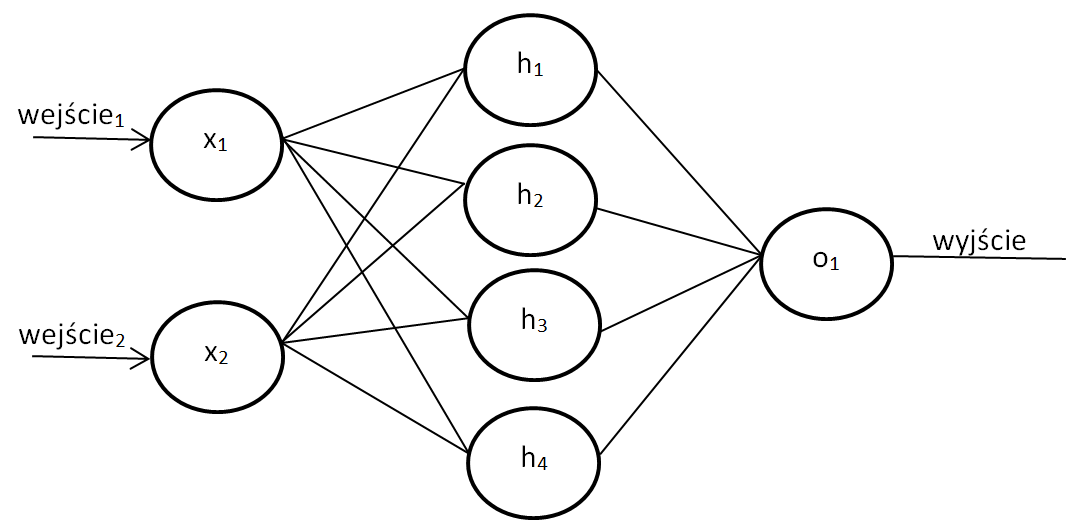
\includegraphics[width=0.7\linewidth]{./include/flow_2_4_1}
\caption{Przepływ informacji w topologii 2-4-1.}
\label{fig:flow_2_4_1}
\end{figure}

Następnie przeprowadzono test sieci w topologi przedstawionej na rysunku \ref{fig:neuro_2_4_1}.

W stosunku do poprzedniego testu, architektura sztucznej sieci neuronowej została rozbudowana o dodatkową warstwę ukrytą. Pozostałe cechy sieci takie jak inicjalizacja wag neuronów oraz funkcja aktywacji pozostały bez zmian.

\begin{figure}[!htbp]
\centering
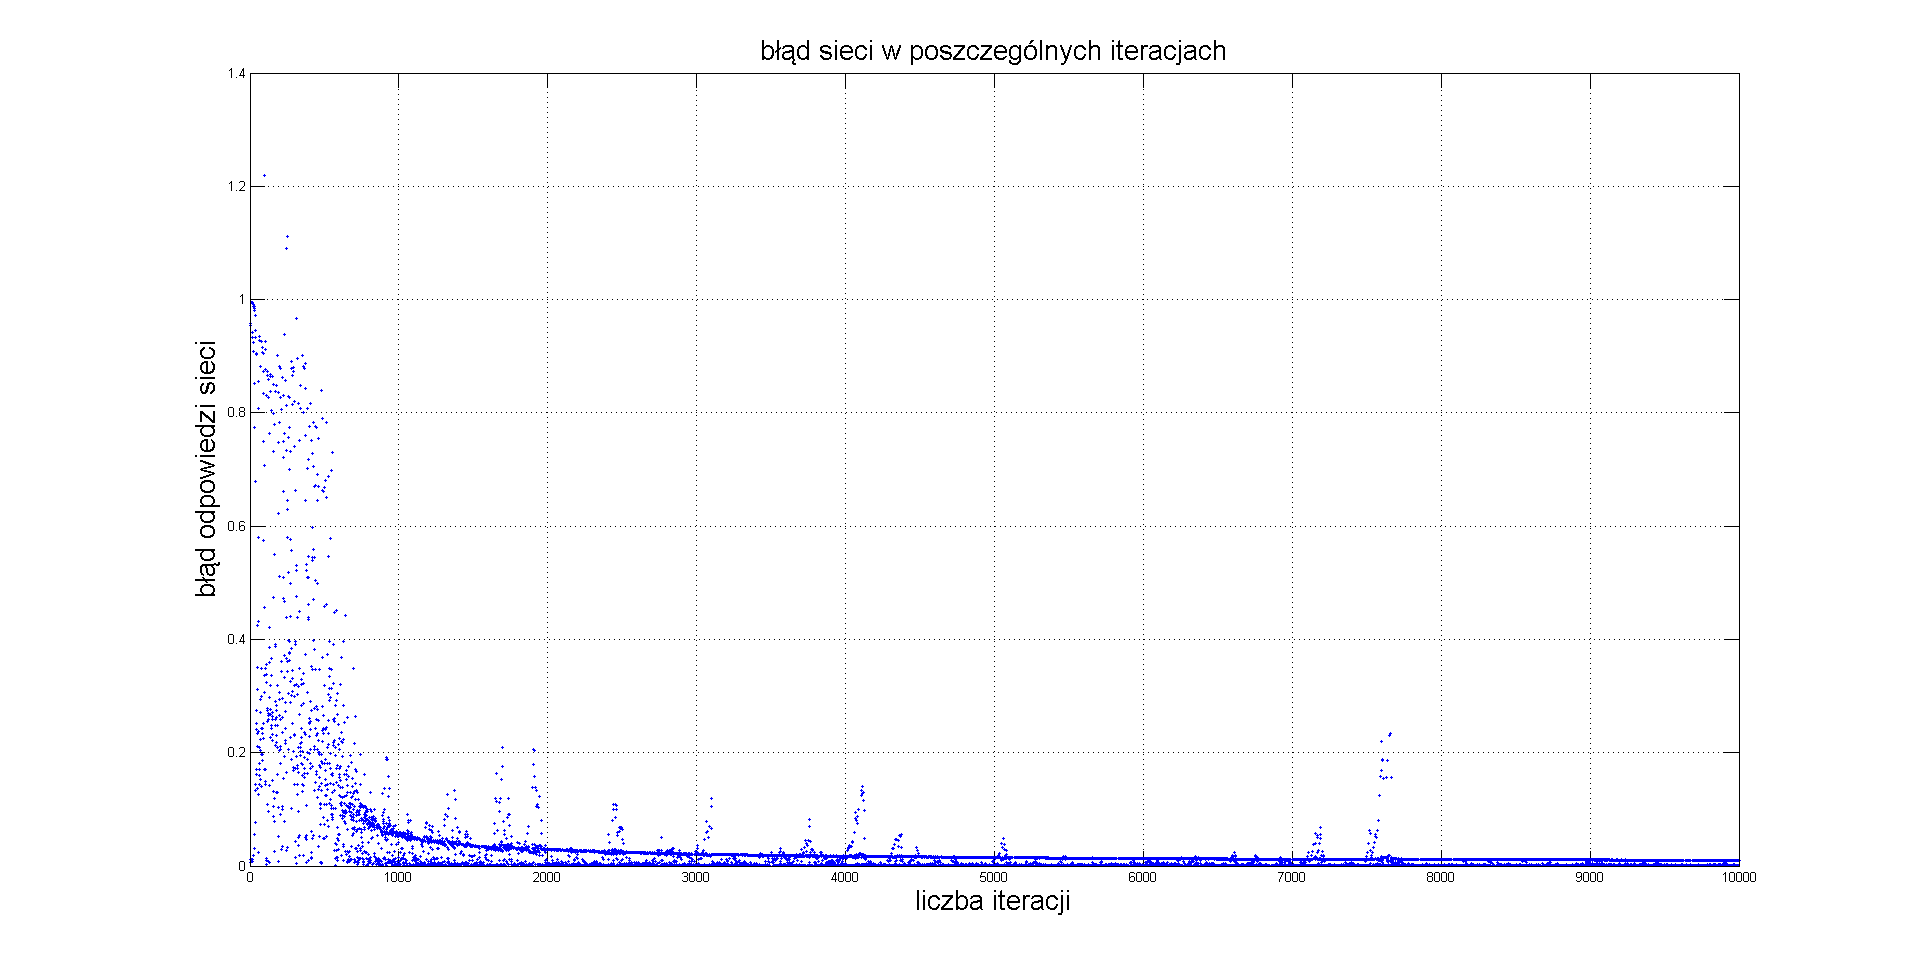
\includegraphics[width=1\linewidth]{./include/topologia_2_4_1}
\caption{Wykres błędu w kolejnych iteracjach dla sieci o topologii 2-4-1.}
\label{fig:neuro_2_4_1}
\end{figure}

%TODO wnioski do uczenia sieci

\begin{table}
\centering

\label{tab:xor_output_2_4_1}
\begin{tabular}{|r|l|l|}
  \hline 
  Wejście 1 & Wejście 2 & Wyjście \\
  \hline 
  0 & 0 & 0 \\
  \hline
  0 & 1 & 1 \\
  \hline
  1 & 0 & 1 \\
  \hline
  1 & 1 & 0 \\
  \hline
\end{tabular}
\caption{Odpowiedzi sieci neuronowej o topologii 2-4-1.}
\end{table}

\section{Testy działania algorytmu sterowania opartego na sztucznej sieci neuronowej}

\chapter{Podsumowanie}
\label{cha:podsumowanie}

% itd.
% \appendix
% \include{dodatekA}
% \include{dodatekB}
% itd.

\bibliographystyle{alpha}
\bibliography{bibliografia}
%\begin{thebibliography}{1}
%
%\bibitem{Dil00}
%A.~Diller.
%\newblock {\em LaTeX wiersz po wierszu}.
%\newblock Wydawnictwo Helion, Gliwice, 2000.
%
%\bibitem{Lam92}
%L.~Lamport.
%\newblock {\em LaTeX system przygotowywania dokumentów}.
%\newblock Wydawnictwo Ariel, Krakow, 1992.
%
%\bibitem{Alvis2011}
%M.~Szpyrka.
%\newblock {\em {On Line Alvis Manual}}.
%\newblock AGH University of Science and Technology, 2011.cccccc
%\newblock \\\texttt{http://fm.ia.agh.edu.pl/alvis:manual}.
%
%\end{thebibliography}

\end{document}
